\section{Worked examples}
\label{sec:worked}

All values in this section were computed by \code{tools/make\_worked\_examples.py} using the reference tool \code{tools/evidence\_hash.py}. The evidence is synthetic but follows the procedures of \cref{sec:classes}. Salts are derived from a fixed demonstration seed so that the numbers are reproducible; in production they are random. The resulting manifests validate against the schema and are in \code{spec/examples/}.

\subsection{Crime-scene photograph: why integrity and identity are different questions}
\Cref{fig:scene} shows the reference photograph, a second photograph of the same scene taken seconds later, and a copy of the reference with the knife digitally removed. \Cref{tab:photo} compares seven variants with the reference by exact hash (L1) and by perceptual hash (L2).

\begin{figure}[htbp]
\centering
\begin{tabular}{ccc}
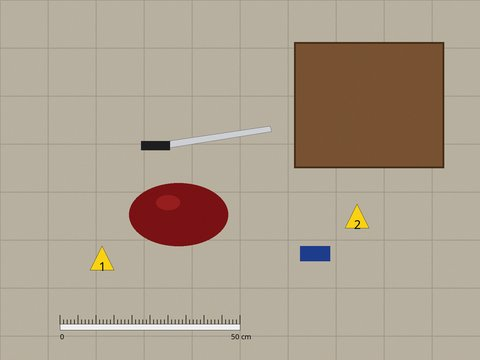
\includegraphics[width=0.31\linewidth]{figures/scene_original.jpg} &
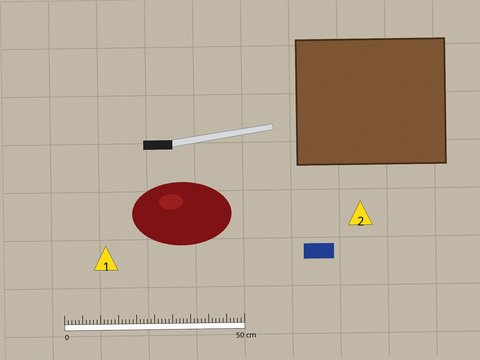
\includegraphics[width=0.31\linewidth]{figures/scene_second.jpg} &
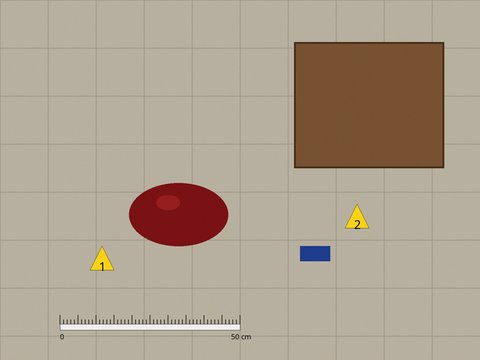
\includegraphics[width=0.31\linewidth]{figures/scene_tampered.jpg} \\
\small (a) reference \code{IMG\_0001} & \small (b) second shot, same scene & \small (c) knife digitally removed
\end{tabular}
\caption{Synthetic scene photographs (reduced).}
\label{fig:scene}
\end{figure}

\begin{table}[htbp]
\centering\small
\begin{tabular}{@{}p{0.30\linewidth}p{0.25\linewidth}cc>{\centering\arraybackslash}p{0.11\linewidth}@{}}
\toprule
Variant of \texttt{IMG\_0001} & SHA-256 (first 16 hex) & L1 equal? & pHash $d_H$ & L2 ($d_H\le 10$)\\
\midrule
Original file as produced by the device & \texttt{0ee55003\allowbreak{}4602fa2d\ldots} & yes & 0 & same\\
Byte-for-byte copy (e.g. to the master-negative disk) & \texttt{0ee55003\allowbreak{}4602fa2d\ldots} & yes & 0 & same\\
Opened and re-saved as JPEG (same quality setting) & \texttt{f769b244\allowbreak{}9ec51305\ldots} & \textbf{no} & 0 & same\\
Only the EXIF date/time edited; pixels untouched & \texttt{c5c6eeca\allowbreak{}12251f4f\ldots} & \textbf{no} & 0 & same\\
Second photograph of the same scene, seconds later & \texttt{81e30dfc\allowbreak{}25a89d1d\ldots} & \textbf{no} & 0 & same\\
Original with the knife digitally removed & \texttt{2e2864e3\allowbreak{}1f9b783b\ldots} & \textbf{no} & 0 & same\\
Photograph of a different scene & \texttt{90ed56c4\allowbreak{}0568ae5a\ldots} & \textbf{no} & 28 & different\\
\bottomrule
\end{tabular}

\caption{Seven variants of a scene photograph compared with the reference by \shatwo{} (L1) and 64-bit DCT pHash (L2).}
\label{tab:photo}
\end{table}

What the table shows:
\begin{itemize}
  \item \textbf{Only a byte-for-byte copy passes L1.} Re-saving with identical settings, or editing one EXIF field without touching a pixel, produces an unrelated \shatwo{}. This is why the SOP insists that recordings are never opened in editing software before hashing~\cite{sopbnss}.
  \item \textbf{A second photograph of the same scene} fails L1, as every new capture must (\enquote{no two photographs are the same}), yet is recognised by L2 (distance \PhotoSecondDist{}).
  \item \textbf{The tampered image passes L2} (distance \PhotoTamperDist{}) and is caught only by L1. Perceptual fingerprints must therefore never be used to establish integrity.
  \item \textbf{A different scene} is far away in L2 (distance \PhotoOtherDist{}).
\end{itemize}

\subsection{Recovered notebook: page scans, Merkle tree, tampering and re-identification}
The notebook (item E004) is documented by a cover photograph, an edge photograph and six lossless page scans at 300~dpi (\cref{fig:notebook}). \Cref{tab:nbart} lists the artefacts, and \cref{tab:nbled} shows what is written to the ledger.

\begin{figure}[htbp]
\centering
\begin{tabular}{cc}
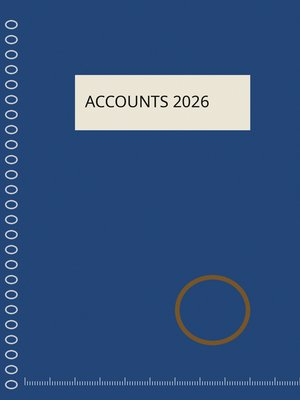
\includegraphics[height=5.2cm]{figures/notebook_cover.jpg} &
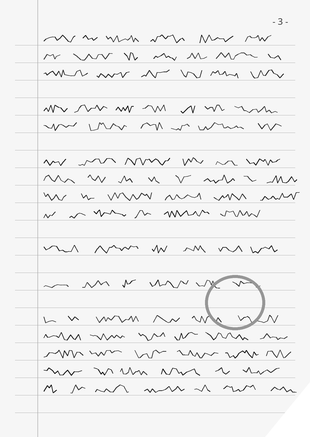
\includegraphics[height=5.2cm]{figures/notebook_page3.png} \\
\small cover photograph (A001) & \small page 3 scan (A005): torn corner, ring stain
\end{tabular}
\caption{Reference captures of the notebook (reduced).}
\label{fig:notebook}
\end{figure}

\begin{table}[htbp]
\centering\small
\begin{tabular}{@{}clll@{}}
\toprule
Artefact & Role & Size (bytes) & SHA-256\\
\midrule
\texttt{A001} & cover\_photo & 326615 & \texttt{fab9701b\allowbreak{}8a921d58\allowbreak{}38fc5c7e\ldots}\\
\texttt{A002} & edge\_photo & 128632 & \texttt{3dedfa67\allowbreak{}c8b545f3\allowbreak{}b0499be1\ldots}\\
\texttt{A003} & page\_scan & 38947 & \texttt{4b83b163\allowbreak{}6bb458bd\allowbreak{}4f1f8ba5\ldots}\\
\texttt{A004} & page\_scan & 41227 & \texttt{c71aed67\allowbreak{}a84ba93a\allowbreak{}6fcad3ab\ldots}\\
\texttt{A005} & page\_scan & 38765 & \texttt{6f56721a\allowbreak{}bffa9ba0\allowbreak{}c1d308ce\ldots}\\
\texttt{A006} & page\_scan & 36499 & \texttt{9d17cf12\allowbreak{}86e73ba1\allowbreak{}fc14b41d\ldots}\\
\texttt{A007} & page\_scan & 38053 & \texttt{76eb8499\allowbreak{}bda3742a\allowbreak{}ac892885\ldots}\\
\texttt{A008} & page\_scan & 43709 & \texttt{b074bdfa\allowbreak{}579c82af\allowbreak{}ca8858cd\ldots}\\
\bottomrule
\end{tabular}

\caption{Notebook artefacts in Merkle-leaf order (SHA-256 truncated).}
\label{tab:nbart}
\end{table}

\begin{table}[htbp]
\centering\small
\begin{tabular}{@{}lp{0.62\linewidth}@{}}
\toprule
Ledger field & Value\\
\midrule
\texttt{evidence\_id} & \texttt{GJ-GNR-CYBPS-2026-000123-E004}\\
\texttt{evidence\_class} & \texttt{PHYSICAL\_DOCUMENT}\\
\texttt{artefact\_count} & 8\\
\texttt{manifest\_sha256} & \texttt{d5b71925\allowbreak{}0e11dda2\allowbreak{}55782f9f\allowbreak{}a1d4b77d\allowbreak{}746ae94d\allowbreak{}7a5bc523\allowbreak{}2df470b2\allowbreak{}e902ade1}\\
\texttt{merkle\_root} & \texttt{6e845149\allowbreak{}4a032e33\allowbreak{}17bc66df\allowbreak{}35c259c9\allowbreak{}68a35e2f\allowbreak{}c67832d4\allowbreak{}f079695e\allowbreak{}9c514102}\\
\bottomrule
\end{tabular}

\caption{Ledger record of the notebook: the only data about E004 replicated on-chain.}
\label{tab:nbled}
\end{table}

\paragraph{Attack 1: a page is substituted in the evidence store.} An insider replaces the scan of page 4 with a scan of a re-written page 4. Verification against the manifest reports:
\begin{itemize}[nosep]
\item A006 (page\_004.png): size\_bytes mismatch: manifest 36499 != file 1140696
\item A006 (page\_004.png): sha256 mismatch: manifest \texttt{9d17cf1286e7\ldots} != file \texttt{2edd917f266b\ldots}
\item A006 (page\_004.png): sha3\_256 mismatch: manifest \texttt{08601e27fb44\ldots} != file \texttt{fef33dd0e7c5\ldots}
\item Merkle root from files mismatch: manifest \texttt{6e8451494a03\ldots} != files \texttt{d2e3ffa44a09\ldots}
\end{itemize}

The exact artefact (A006, page 4) is identified, and the Merkle root recomputed from the files no longer matches.

\paragraph{Attack 2: the insider also rewrites the manifest.} The manifest is now internally consistent with the forged page, but it no longer matches the ledger:
\begin{itemize}[nosep]
\item Manifest hash mismatch: ledger \texttt{d5b719250e11\ldots} != manifest \texttt{ffd436514d57\ldots}
\item Merkle root mismatch: ledger \texttt{6e8451494a03\ldots} != manifest \texttt{d2e3ffa44a09\ldots}
\end{itemize}

Defeating this would require changing the ledger record, which needs a BFT quorum of agencies (\cref{sec:network}).

\paragraph{Selective disclosure.} To show a court only page 4, the custodian discloses that page, its salt and the inclusion proof in \cref{tab:proof}. The verifier recomputes the leaf and the path and obtains the ledger's Merkle root without seeing any other page.

\begin{table}[htbp]
\centering\small
\begin{tabular}{@{}ll@{}}
\toprule
Leaf (artefact) & \texttt{A006} (page 4), index 5 of 8\\
Leaf salt & \texttt{3d4e9066\allowbreak{}c4cdde07\allowbreak{}f02e0b2a\allowbreak{}fee9a8e9\ldots}\\
Artefact SHA-256 & \texttt{9d17cf12\allowbreak{}86e73ba1\allowbreak{}fc14b41d\allowbreak{}ad74b931\ldots}\\
Audit path [0] & \texttt{f6406262\allowbreak{}fac99752\allowbreak{}72a7909c\allowbreak{}44f361d2\ldots}\\
Audit path [1] & \texttt{f554525c\allowbreak{}9214f3fe\allowbreak{}ee254972\allowbreak{}21aa3293\ldots}\\
Audit path [2] & \texttt{55fba80e\allowbreak{}03452a81\allowbreak{}83405fce\allowbreak{}cc05bb60\ldots}\\
Merkle root & \texttt{6e845149\allowbreak{}4a032e33\allowbreak{}17bc66df\allowbreak{}35c259c9\ldots}\\
Proof verifies & yes\\
\bottomrule
\end{tabular}

\caption{RFC 6962 inclusion proof for page 4 (hashes truncated). Three sibling hashes suffice for eight leaves.}
\label{tab:proof}
\end{table}

\paragraph{Re-identification at the FSL.} On receipt, all six sides are re-scanned on a different scanner. \Cref{tab:nbrescan} shows that every \shatwo{} differs, as expected, while the perceptual distances stay at or below \NbRescanMaxDist{}. The substituted page lies at distance \NbForgedDist{} and is rejected.

\begin{table}[htbp]
\centering\small
\begin{tabular}{@{}c>{\raggedright}p{0.24\linewidth}llcc@{}}
\toprule
Page & Comparison & Original scan & New scan & $d_H$ & L2 verdict\\
\midrule
1 & FSL re-scan of the same page & \texttt{4b83b163\allowbreak{}6bb4\ldots} & \texttt{7d1dd5a3\allowbreak{}49b1\ldots} & 4 & MATCH\\
2 & FSL re-scan of the same page & \texttt{c71aed67\allowbreak{}a84b\ldots} & \texttt{7b0b17e3\allowbreak{}4823\ldots} & 4 & MATCH\\
3 & FSL re-scan of the same page & \texttt{6f56721a\allowbreak{}bffa\ldots} & \texttt{a7b2fb28\allowbreak{}17d6\ldots} & 2 & MATCH\\
4 & FSL re-scan of the same page & \texttt{9d17cf12\allowbreak{}86e7\ldots} & \texttt{a2267f0a\allowbreak{}d4b9\ldots} & 4 & MATCH\\
5 & FSL re-scan of the same page & \texttt{76eb8499\allowbreak{}bda3\ldots} & \texttt{b95f550f\allowbreak{}b362\ldots} & 2 & MATCH\\
6 & FSL re-scan of the same page & \texttt{b074bdfa\allowbreak{}579c\ldots} & \texttt{ee4a979f\allowbreak{}22b2\ldots} & 2 & MATCH\\
4 & Substituted (re-written) page 4 & \texttt{9d17cf12\allowbreak{}86e7\ldots} & \texttt{2edd917f\allowbreak{}266b\ldots} & 20 & \textbf{NO MATCH}\\
\bottomrule
\end{tabular}

\caption{L2 re-identification of the notebook pages (threshold $d_H \le 10$).}
\label{tab:nbrescan}
\end{table}

\subsection{Physical item: 3D scan of a knife}
The knife (item E002) is documented by a structured-light scan of \KnifeRefPoints{} points (\cref{fig:knife}). Re-scans are taken in a new pose, with new sampling and 0.15~mm sensor noise, then aligned by ICP and compared symmetrically (\cref{tab:knife}).

\begin{figure}[htbp]
\centering
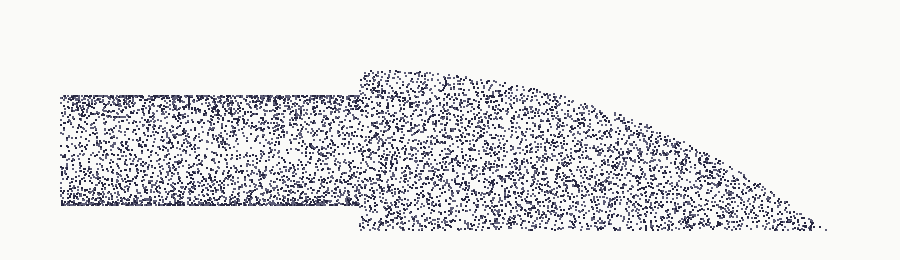
\includegraphics[width=0.75\linewidth]{figures/knife_scan_top.png}
\caption{Reference 3D scan of the knife (top view of the point cloud).}
\label{fig:knife}
\end{figure}

\begin{table}[htbp]
\centering\small
\begin{tabular}{@{}p{0.46\linewidth}cccc@{}}
\toprule
Query scan compared with the reference scan & RMS (mm) & P95 (mm) & Max (mm) & L2 verdict\\
\midrule
Same knife, re-scanned at FSL (new pose, new sampling, 0.15 mm noise) & 0.568 & 0.965 & 2.386 & MATCH\\
Same knife after an 8 x 5 mm nick appeared in the edge & 0.579 & 0.975 & 4.444 & \textbf{NO MATCH}\\
Same knife with 6 mm of the tip broken off & 0.570 & 0.964 & 5.024 & \textbf{NO MATCH}\\
Look-alike knife, blade 6 mm longer & 0.581 & 0.982 & 4.365 & \textbf{NO MATCH}\\
\bottomrule
\end{tabular}

\caption{3D-scan re-identification (rule: RMS $\le$ \KnifeRuleRms{} mm and maximum $\le$ \KnifeRuleMax{} mm).}
\label{tab:knife}
\end{table}

The RMS barely changes across all four cases, because it is dominated by sampling density, so a small local defect hardly moves it. The \emph{maximum} symmetric deviation is what reveals the 8$\times$5~mm nick, the broken tip and the 6~mm longer look-alike. Two lessons follow. The metric must be symmetric and must include a local term. And thresholds must be calibrated against the scanner's own repeatability: here the honest re-scan reaches a maximum of about 2.4~mm purely from sampling.

\subsection{Forensic image: acquisition verification and damage localisation}
\begin{table}[htbp]
\centering\small
\begin{tabular}{@{}ll@{}}
\toprule
Quantity & Value\\
\midrule
Source media size & 8{,}388{,}608 bytes (8 MiB)\\
SHA-256 of bit stream read during acquisition & \texttt{1b3166fa\allowbreak{}49149b5c\allowbreak{}3a2370e9\allowbreak{}d4242e60\ldots}\\
SHA-256 recomputed from finished image & \texttt{1b3166fa\allowbreak{}49149b5c\allowbreak{}3a2370e9\allowbreak{}d4242e60\ldots}\\
Acquisition verified (stream = image) & yes\\
SHA-256 of working copy with 1 bit flipped at byte 5{,}000{,}000 & \texttt{84b6d634\allowbreak{}e07837f5\allowbreak{}1604d601\allowbreak{}496e7489\ldots}\\
Chunk Merkle root (1 MiB chunks), good image & \texttt{e34fb65d\allowbreak{}b1bfba88\allowbreak{}0d50220a\allowbreak{}a447df5e\ldots}\\
Chunk Merkle root, corrupted copy & \texttt{bde2bf07\allowbreak{}c5c6c89d\allowbreak{}e6b98a40\allowbreak{}b8898912\ldots}\\
Chunks that differ (0-based) & 4 (bytes 4{,}194{,}304--5{,}242{,}879)\\
\bottomrule
\end{tabular}

\caption{Acquisition of an 8 MiB medium; a single bit flipped later in a working copy.}
\label{tab:disk}
\end{table}

The acquisition is verified when the hash of the stream read from the source equals the hash of the finished image. A single flipped bit in a later working copy changes the whole-file hash completely. The chunk Merkle tree localises the damage to one 1~MiB chunk, so the rest of the copy can still be shown to be intact.
